\section{Motor Testing}\label{Motor Testing_Appendix}
For designing the controller, it is important to have accurate values and constants for the motors used in the drone if you want to accurately determine and calculate its position in the physical space. The motors used for the project did not have a data sheet available with motor constants/characteristics, so testing would have to be done to determine these values.  motor constants relevant for this project include, “Motor velocity constant” ($K_v$) and “Motor torque constant” ($K_T$)
\subsection{Test Setup}
For the test setup the following items were used:
\begin{itemize}
    \item A photo sensor (to measure RPM)
    \item Marked Propeller
    \item One coreless dc motor of unknown origin.
    \item A vise
    \item AFD-8896 Mosfet
    \item Seeed xiao ble nrf52840 sense 
    \item Power supply
\end{itemize}

The photo sensor works by measuring a change in light reflection, so a white propeller was marked with black touché to create an RPM measuring tool. The motor with the propeller is mounted to a table with a vise to reduce vibration.
To test using PWM, the motor is turned on through the Seeed, so the rpm can be measured and changed. All the values are recorded 3 times for each PWM to increase consistency in the measurements. The motor can handle inputs at both 3.7V and 4.2V, so the test was done with both voltages, since the battery output will be somewhere in between depending on the discharge. The voltage the motor draws is measured through a multimeter. \\

The Seeed is used to control the PWM but cannot alone supply enough current to power the motor, therefore the power is provided directly through the power supply and controlled through a mosfet. At lower values of PWM however, the gate on the mosfet will close so the motor will not turn on.

\subsection{Theory}
Motor velocity- or motor speed constant is measured in RPM per volt and can be calculated by taking the motors unloaded rotational speed divided by the peak voltage. It was necessary to load the motor slightly, to measure using a photosensor. The small load is therefore deemed negligible.\\
 
The motor speed constant can then be used to calculate the motor torque constant, which is measured in newton meter per ampere. This constant will be important for the model to determine the change in thrust needed to achieve the desired outcome.\cite{MotorConstants} \\ 

\begin{figure}[H]
\begin{center}
   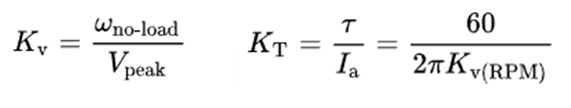
\includegraphics[scale =1]{pictures/control/Motor constants theory.png}
\end{center}
\caption{Motor Constant Equations}
\end{figure}

The test was also done to determine the thrust coefficient of the motor. Using the thrust testing from before, the thrust can be determined based on the voltage drop. Then, by converting the RPM to angular velocity, it is possible to derive the thrust coefficient by dividing the thrust with the angular velocity.
For both the motor constants and values used to calculate the constants are from tests with 3.0V inputs, which is the voltage needed to achieve the theoretical hover thrust. This is sensible since most of the time the drone will be operating around these values. 

\subsection{Data}
Some data could not be gathered from the setup since the motor was outputting too high an RPM to be measured with the equipment. And the lower PWM missing values is because of the mosfet closing.

\begin{figure}[H]
\begin{center}
   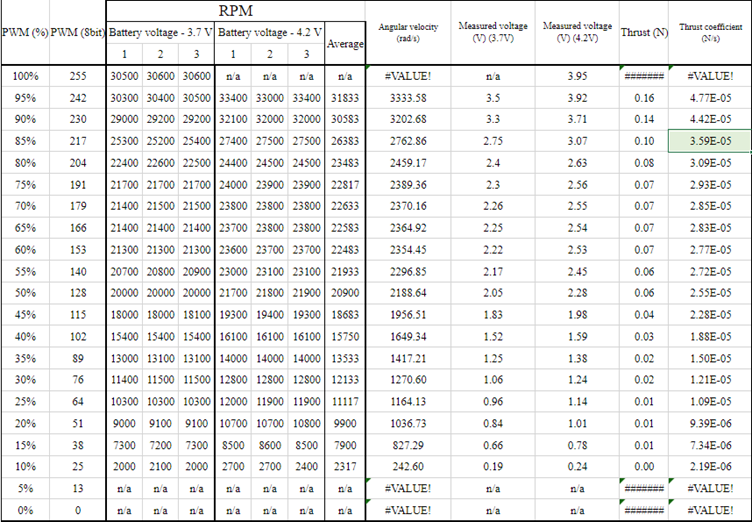
\includegraphics[scale =0.8]{pictures/control/BigData.png}
\end{center}
\caption{Testing Data with Thrust Coefficient highlighted in green}
\end{figure}

\subsection{Conclusion of Theory}

\begin{figure}[H]
\begin{center}
   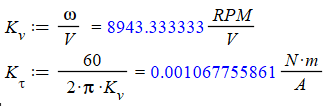
\includegraphics[scale =1]{pictures/control/Motor constants calc.png}
\end{center}
\caption{Motor Constants}
\end{figure}